\documentclass[UTF8,a4paper,12pt]{ctexart}

\usepackage{geometry}
\geometry{left=2.4cm,right=2.4cm,top=2.5cm,bottom=2.5cm}

\usepackage{graphicx}
\usepackage{booktabs}
\usepackage{longtable}
\usepackage{array}
\usepackage{float}
\usepackage{subcaption}
\usepackage{amsmath}
\usepackage{hyperref}
\usepackage{xcolor}

\graphicspath{{figures/}}

\hypersetup{
    colorlinks=true,
    linkcolor=blue,
    urlcolor=blue
}

\title{股票快照价格移动方向预测项目\\EDA 探索性数据分析报告}
\author{}
\date{}

\begin{document}

\maketitle

\section{EDA 目标}

本次探索性数据分析（Explatory Data Analysis, EDA）的目标是在进入特征工程和建模之前，系统检查股票快照数据的完整性、字段结构、数据质量、订单簿合理性、标签分布以及潜在异常。该项目的核心任务是：基于股票订单簿快照数据，预测未来 5、10、20、40、60 个 tick 后的中间价移动方向。

EDA 阶段重点回答以下问题：

\begin{enumerate}
    \item 数据文件是否完整，是否存在缺失交易日、缺失标的或缺失 session；
    \item 原始 CSV 文件是否能够正常读取，是否存在空文件或读取失败文件；
    \item 字段是否符合任务说明，是否存在缺失字段或字段命名差异；
    \item 数据是否存在缺失值、重复行、无穷值等基础质量问题；
    \item 订单簿价格与挂单量是否满足基本金融逻辑；
    \item \texttt{n\_midprice} 是否与买一价、卖一价规则基本一致；
    \item 标签是否确实表示“未来 N 个 tick 的价格移动方向”；
    \item 标签是否存在类别不均衡，后续建模是否需要加权或重采样；
    \item 哪些变量需要在特征工程阶段进行变换或异常处理。
\end{enumerate}

\section{数据概览}

\begin{table}[H]
\centering
\caption{数据文件与样本概览}
\begin{tabular}{lr}
\toprule
指标 & 结果 \\
\midrule
理论文件组合数 & 1580 \\
实际读取文件数 & 1521 \\
成功读取文件数 & 1521 \\
读取失败文件数 & 0 \\
空文件数 & 0 \\
缺失文件组合数 & 59 \\
异常额外文件组合数 & 0 \\
总样本行数 & 3,040,479 \\
总字段数 & 35 \\
\bottomrule
\end{tabular}
\end{table}

理论上，数据应包含 10 只股票、79 个交易日、上午与下午两个交易时段，因此理论文件组合数为：
\[
10 \times 79 \times 2 = 1580.
\]
实际读取到 1521 个文件，说明存在 59 个股票-日期-session 组合缺失。该问题不会阻止后续建模，但在时间序列划分和样本构造时需要注意，避免默认所有股票在所有日期都有完整数据。

\begin{figure}[H]
\centering
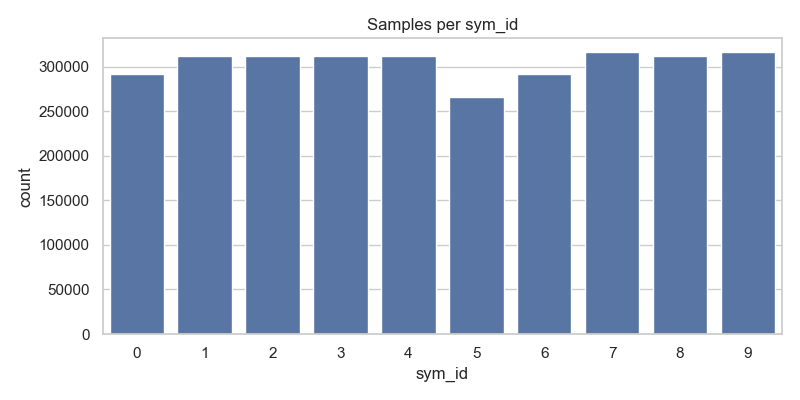
\includegraphics[width=0.88\textwidth]{samples_per_sym.png}
\caption{不同股票样本量分布}
\label{fig:samples_per_sym}
\end{figure}

从图 \ref{fig:samples_per_sym} 可以看出，不同 \texttt{sym\_id} 的样本量总体接近，说明 10 只股票的样本覆盖较均衡。不过，\texttt{sym\_id=5} 的样本量相对较少，后续可以关注该标的是否存在更多缺失交易 session。

\begin{figure}[H]
\centering
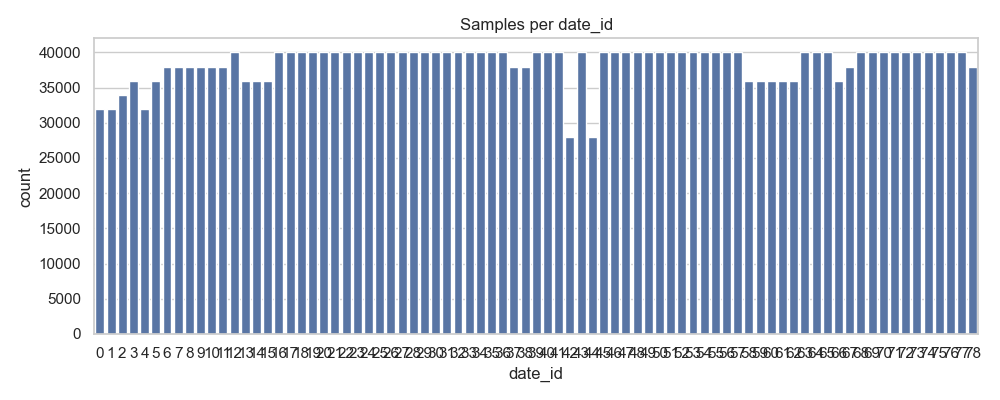
\includegraphics[width=0.95\textwidth]{samples_per_date.png}
\caption{不同日期样本量分布}
\label{fig:samples_per_date}
\end{figure}

图 \ref{fig:samples_per_date} 显示，大多数日期的样本量接近 40,000，但部分日期样本量明显偏低。这与缺失 59 个文件组合的结论一致，说明部分交易日可能存在缺失股票或缺失 session。

\begin{figure}[H]
\centering
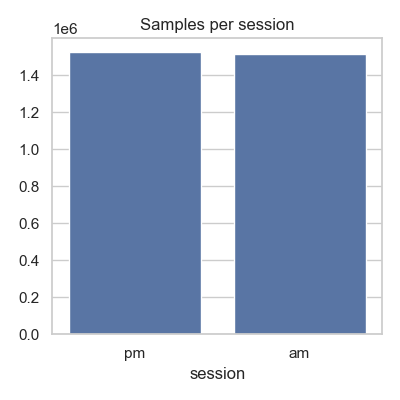
\includegraphics[width=0.55\textwidth]{samples_per_session.png}
\caption{上午/下午 session 样本量分布}
\label{fig:samples_per_session}
\end{figure}

图 \ref{fig:samples_per_session} 显示，上午和下午 session 的样本量总体接近，说明两个交易时段的数据覆盖较为平衡。

\section{字段说明与字段检查}

实际数据包含 35 个字段，核心字段包括表 \ref{tab:fields} 所示内容。

\begin{table}[H]
\centering
\caption{核心字段说明}
\label{tab:fields}
\begin{tabular}{ll}
\toprule
字段类型 & 字段 \\
\midrule
标识字段 & \texttt{date}, \texttt{time}, \texttt{sym} \\
最新价字段 & \texttt{n\_close} \\
成交字段 & \texttt{amount\_delta} \\
中间价字段 & \texttt{n\_midprice} \\
买盘价格字段 & \texttt{n\_bid1} 至 \texttt{n\_bid5} \\
买盘挂单量字段 & \texttt{n\_bsize1} 至 \texttt{n\_bsize5} \\
卖盘价格字段 & \texttt{n\_ask1} 至 \texttt{n\_ask5} \\
卖盘挂单量字段 & \texttt{n\_asize1} 至 \texttt{n\_asize5} \\
标签字段 & \texttt{label\_5}, \texttt{label\_10}, \texttt{label\_20}, \texttt{label\_40}, \texttt{label\_60} \\
\bottomrule
\end{tabular}
\end{table}

需要注意的是，实际数据中最新价字段为 \texttt{n\_close}，而不是部分说明中出现的 \texttt{close}；标签字段使用下划线命名，即 \texttt{label\_5}、\texttt{label\_10} 等。

\section{数据质量检查}

\begin{table}[H]
\centering
\caption{基础数据质量检查}
\begin{tabular}{lr}
\toprule
检查项 & 结果 \\
\midrule
缺失值 & 未发现明显缺失值 \\
重复行数 & 0 \\
Inf / -Inf & 未发现 \\
读取失败文件 & 0 \\
空文件 & 0 \\
\bottomrule
\end{tabular}
\end{table}

基础数据质量较好，未发现缺失值、重复行或无穷值。这说明后续可以直接进入异常检查、特征工程与建模准备，而不需要大规模处理缺失值。

\section{订单簿异常检查}

订单簿数据需要满足基本的价格层级关系。正常情况下，一般应有：
\[
n\_bid1 \leq n\_ask1.
\]
买盘内部应满足：
\[
n\_bid1 \geq n\_bid2 \geq n\_bid3 \geq n\_bid4 \geq n\_bid5.
\]
卖盘内部应满足：
\[
n\_ask1 \leq n\_ask2 \leq n\_ask3 \leq n\_ask4 \leq n\_ask5.
\]

\begin{table}[H]
\centering
\caption{订单簿主要异常统计}
\begin{tabular}{lrr}
\toprule
异常类型 & 数量 & 比例 \\
\midrule
\texttt{n\_bid1 > n\_ask1} & 30,853 & 1.01\% \\
\texttt{n\_bid2 > n\_ask2} & 32,468 & 1.07\% \\
\texttt{n\_bid3 > n\_ask3} & 33,806 & 1.11\% \\
\texttt{n\_bid4 > n\_ask4} & 34,696 & 1.14\% \\
\texttt{n\_bid5 > n\_ask5} & 35,674 & 1.17\% \\
\texttt{n\_bid2 > n\_bid1} & 308 & 0.01\% \\
\texttt{n\_bid3 > n\_bid2} & 170 & 0.01\% \\
\texttt{n\_bid4 > n\_bid3} & 88 & 约 0.00\% \\
\texttt{n\_bid5 > n\_bid4} & 54 & 约 0.00\% \\
\texttt{n\_ask2 < n\_ask1} & 1,307 & 0.04\% \\
\texttt{n\_ask3 < n\_ask2} & 1,168 & 0.04\% \\
\texttt{n\_ask4 < n\_ask3} & 802 & 0.03\% \\
\texttt{n\_ask5 < n\_ask4} & 924 & 0.03\% \\
size 字段负数 & 0 & 0.00\% \\
\bottomrule
\end{tabular}
\end{table}

结果显示，买卖盘档位内部错序比例很低，挂单量字段也没有负值，说明订单簿结构总体合理。但约 1.01\% 的样本出现 \texttt{n\_bid1 > n\_ask1}，即 crossed book 现象。该比例不算特别高，但后续特征工程时建议保留一个异常标记特征：
\[
is\_crossed\_book = \mathbf{1}(n\_bid1 > n\_ask1),
\]
并在建模阶段比较“保留异常样本”和“过滤异常样本”两种方案的表现。

\begin{figure}[H]
\centering
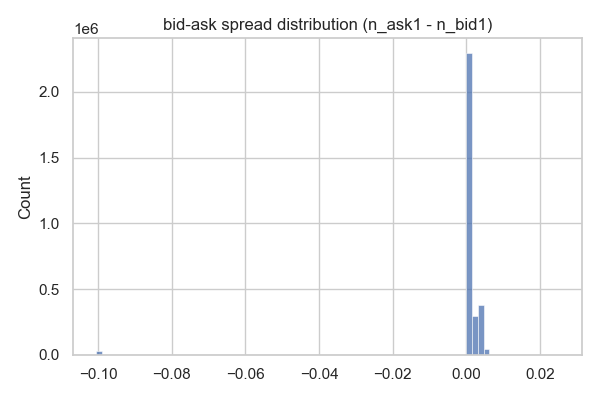
\includegraphics[width=0.76\textwidth]{spread_hist.png}
\caption{原始 bid-ask spread 分布}
\label{fig:spread_hist}
\end{figure}

图 \ref{fig:spread_hist} 显示，大部分样本集中在 0 附近，但存在一部分负 spread，说明确实存在 crossed book 或报价异常。

\begin{figure}[H]
\centering
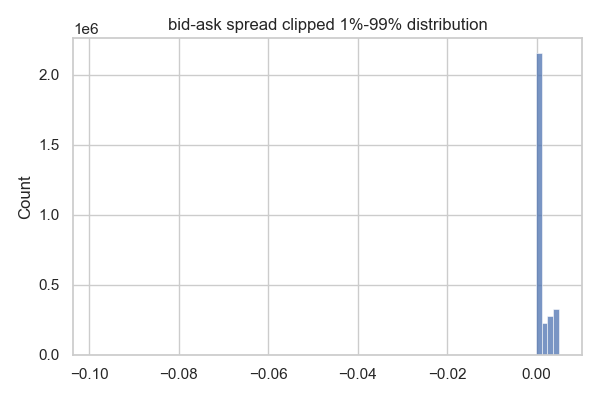
\includegraphics[width=0.76\textwidth]{spread_clipped_hist.png}
\caption{截尾后的 bid-ask spread 分布}
\label{fig:spread_clipped_hist}
\end{figure}

图 \ref{fig:spread_clipped_hist} 更清楚地显示了主体分布。多数样本的 spread 非常接近 0，表明高频快照中买一卖一价格差通常较小。

\section{Midprice 规则检查}

数据说明中给出的中间价规则为：

\begin{enumerate}
    \item 若 \texttt{n\_bid1} 与 \texttt{n\_ask1} 均不为 0，则：
    \[
    n\_midprice = \frac{n\_bid1+n\_ask1}{2};
    \]
    \item 若仅一方不为 0，则中间价取不为 0 的价格；
    \item 若两方均为 0，则置为缺失。
\end{enumerate}

对照该规则重新计算 \texttt{calc\_midprice} 后，与原始 \texttt{n\_midprice} 比较，得到表 \ref{tab:midprice_check}。

\begin{table}[H]
\centering
\caption{Midprice 规则检查结果}
\label{tab:midprice_check}
\begin{tabular}{lr}
\toprule
指标 & 结果 \\
\midrule
mismatch count & 166,530 \\
mismatch ratio & 5.48\% \\
mean absolute difference & \(7.28\times 10^{-5}\) \\
max absolute difference & 0.00545 \\
\bottomrule
\end{tabular}
\end{table}

约 5.48\% 的样本中，数据自带的 \texttt{n\_midprice} 与根据 \texttt{n\_bid1}、\texttt{n\_ask1} 重算结果存在差异。但平均绝对差异较小，说明大部分差异幅度有限。可能原因包括浮点数精度、原始数据源计算方式不同、bid/ask 为 0 时的特殊处理、crossed book 状态或快照对齐方式差异。

后续建模建议优先使用数据自带的 \texttt{n\_midprice}，不要直接用重新计算的值覆盖它。可以额外构造 \texttt{midprice\_diff} 作为数据质量或异常状态特征。

\begin{figure}[H]
\centering
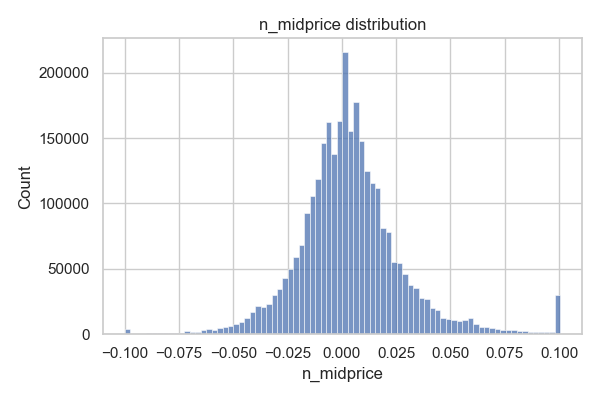
\includegraphics[width=0.78\textwidth]{n_midprice_hist.png}
\caption{\texttt{n\_midprice} 分布}
\label{fig:n_midprice_hist}
\end{figure}

图 \ref{fig:n_midprice_hist} 显示，\texttt{n\_midprice} 分布以 0 为中心，主体分布较集中，符合涨跌幅标准化后的价格特征。在 \(-0.1\) 与 \(0.1\) 附近存在少量样本聚集，可能与涨跌停限制或边界截断有关。

\section{\texttt{amount\_delta} 分布分析}

\texttt{amount\_delta} 表示从上一个 tick 到当前 tick 发生的成交金额变化。该字段分布极度右偏，存在少数极端大值。

\begin{figure}[H]
\centering
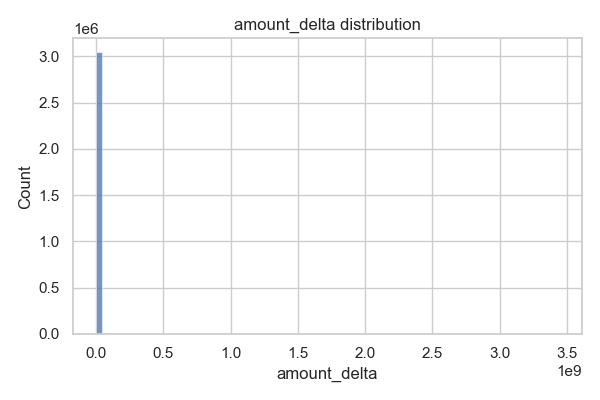
\includegraphics[width=0.78\textwidth]{amount_delta_hist.png}
\caption{原始 \texttt{amount\_delta} 分布}
\label{fig:amount_delta_hist}
\end{figure}

图 \ref{fig:amount_delta_hist} 几乎被极端值拉伸，绝大多数样本挤在 0 附近，说明直接使用原始 \texttt{amount\_delta} 可能会影响模型稳定性。

\begin{figure}[H]
\centering
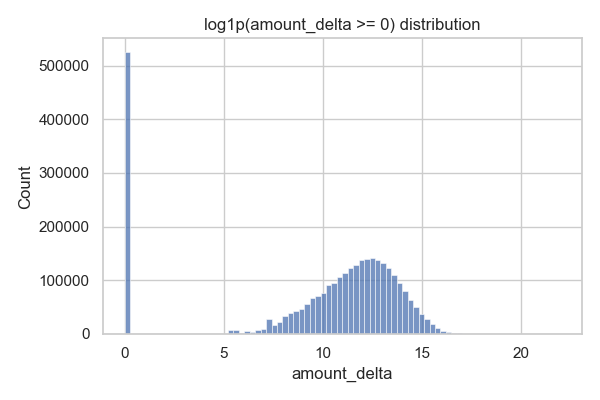
\includegraphics[width=0.78\textwidth]{log_amount_delta_hist.png}
\caption{\texttt{log1p(amount\_delta)} 分布}
\label{fig:log_amount_delta_hist}
\end{figure}

经过 \texttt{log1p} 变换后，主体分布更加清晰。因此后续特征工程建议使用：
\[
log\_amount\_delta = \log(1+\max(amount\_delta,0)),
\]
以降低极端值影响。

\section{标签方向检查}

项目目标是根据当前及过去快照数据，预测未来 N 个 tick 的中间价移动方向。为确认标签方向，对每个文件内部分别检查两种定义：

未来方向：
\[
x_t = n\_midprice_{t+N} - n\_midprice_t.
\]

过去方向：
\[
x_t = n\_midprice_t - n\_midprice_{t-N}.
\]

标签规则为：
\[
\phi(x)=
\begin{cases}
0, & x < -\alpha,\\
1, & -\alpha \le x \le \alpha,\\
2, & x > \alpha.
\end{cases}
\]
其中，\(N=5,10\) 时 \(\alpha=0.0005\)，\(N=20,40,60\) 时 \(\alpha=0.001\)。

检查结果显示，五个标签均与未来方向完全匹配。

\begin{table}[H]
\centering
\caption{标签方向检查结果}
\begin{tabular}{lrl}
\toprule
标签 & future match ratio & 结论 \\
\midrule
\texttt{label\_5} & 1.0000 & 未来方向 \\
\texttt{label\_10} & 1.0000 & 未来方向 \\
\texttt{label\_20} & 1.0000 & 未来方向 \\
\texttt{label\_40} & 1.0000 & 未来方向 \\
\texttt{label\_60} & 1.0000 & 未来方向 \\
\bottomrule
\end{tabular}
\end{table}

因此，后续建模目标可以明确为：使用当前及过去 100 个 tick 的快照特征，预测未来 5、10、20、40、60 个 tick 的中间价移动方向。

\section{标签分布分析}

五个预测窗口的标签分布如表 \ref{tab:label_dist} 所示。

\begin{table}[H]
\centering
\caption{标签分布统计}
\label{tab:label_dist}
\begin{tabular}{lrrr}
\toprule
标签 & 下跌 0 & 不变 1 & 上涨 2 \\
\midrule
\texttt{label\_5} & 460,804 / 15.16\% & 2,122,348 / 69.80\% & 457,327 / 15.04\% \\
\texttt{label\_10} & 647,453 / 21.29\% & 1,762,358 / 57.96\% & 630,668 / 20.74\% \\
\texttt{label\_20} & 520,965 / 17.13\% & 2,006,167 / 65.98\% & 513,347 / 16.88\% \\
\texttt{label\_40} & 741,438 / 24.39\% & 1,586,710 / 52.19\% & 712,331 / 23.43\% \\
\texttt{label\_60} & 857,580 / 28.21\% & 1,361,229 / 44.77\% & 821,670 / 27.02\% \\
\bottomrule
\end{tabular}
\end{table}

可以看出，短窗口 \texttt{label\_5} 中“不变”类占比最高，达到 69.80\%。随着预测窗口变长，价格发生明显移动的比例整体上升，\texttt{label\_60} 是五个任务中类别最均衡的标签。

需要注意的是，\texttt{label\_20} 的“不变”类比例高于 \texttt{label\_10}，这是因为 \(N=20,40,60\) 时阈值 \(\alpha=0.001\)，比 \(N=5,10\) 的阈值 \(0.0005\) 更大，因此更多小幅波动会被归入“不变”类。

\begin{figure}[H]
\centering
\begin{subfigure}{0.48\textwidth}
\centering
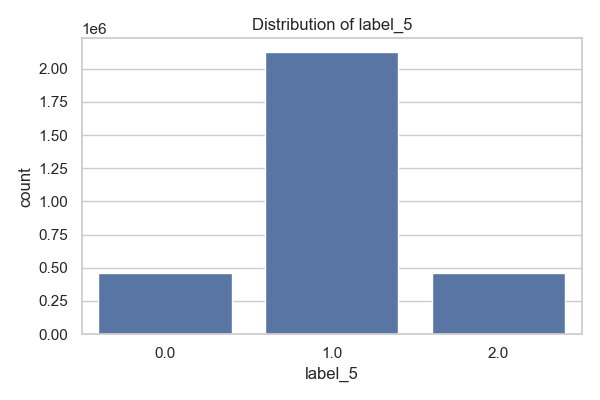
\includegraphics[width=\textwidth]{label_5_distribution.png}
\caption{\texttt{label\_5}}
\end{subfigure}
\hfill
\begin{subfigure}{0.48\textwidth}
\centering
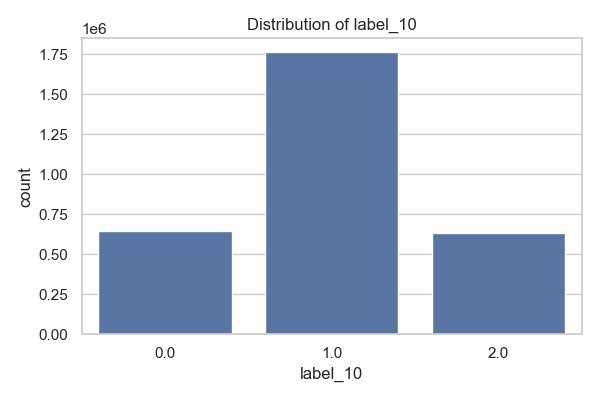
\includegraphics[width=\textwidth]{label_10_distribution.png}
\caption{\texttt{label\_10}}
\end{subfigure}

\vspace{0.4cm}

\begin{subfigure}{0.48\textwidth}
\centering
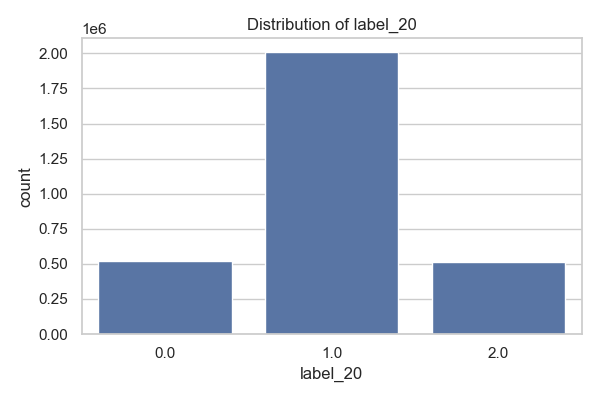
\includegraphics[width=\textwidth]{label_20_distribution.png}
\caption{\texttt{label\_20}}
\end{subfigure}
\hfill
\begin{subfigure}{0.48\textwidth}
\centering
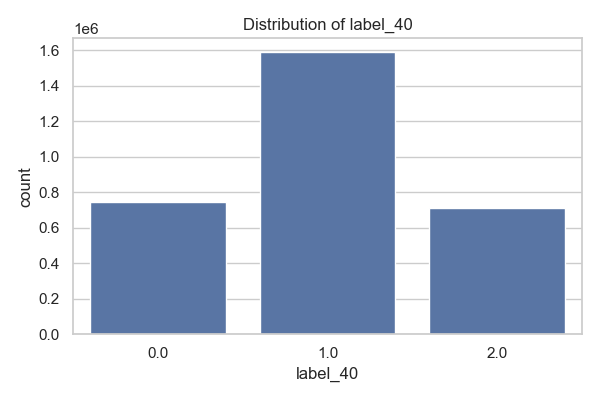
\includegraphics[width=\textwidth]{label_40_distribution.png}
\caption{\texttt{label\_40}}
\end{subfigure}

\vspace{0.4cm}

\begin{subfigure}{0.55\textwidth}
\centering
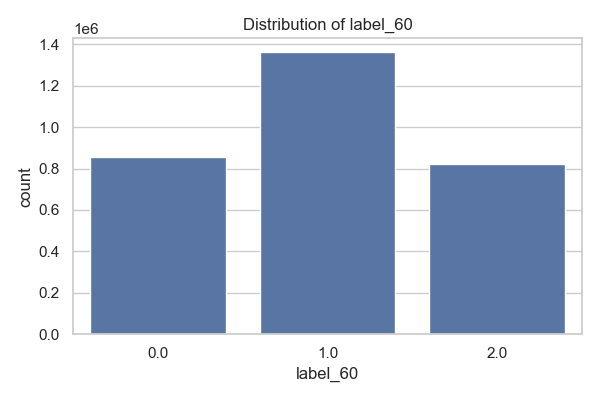
\includegraphics[width=\textwidth]{label_60_distribution.png}
\caption{\texttt{label\_60}}
\end{subfigure}
\caption{五个预测窗口的标签分布}
\label{fig:label_distributions}
\end{figure}

标签分布说明后续训练不能只看 accuracy。尤其在 \texttt{label\_5} 和 \texttt{label\_20} 中，如果模型倾向于预测类别 1，虽然准确率可能较高，但对上涨和下跌方向的预测价值有限。后续评估应重点关注类别 0 和类别 2 的 precision、recall 与 F0.5。

\section{数值字段相关性分析}

\begin{figure}[H]
\centering
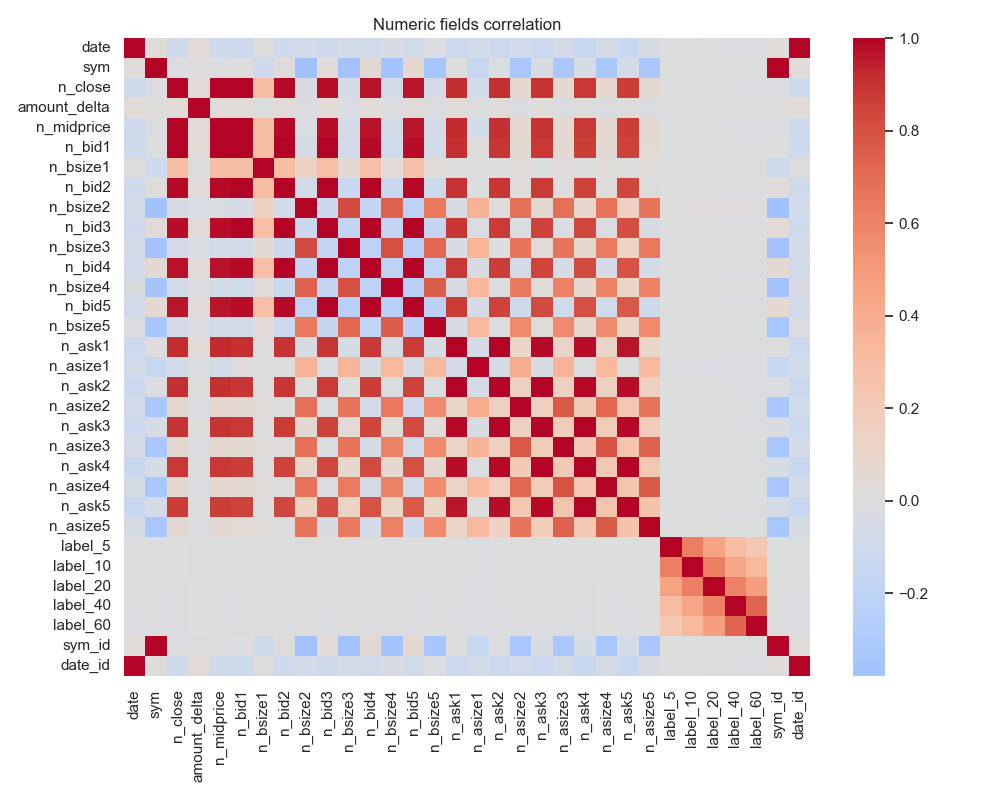
\includegraphics[width=0.95\textwidth]{correlation_heatmap.png}
\caption{主要数值字段相关性热力图}
\label{fig:correlation_heatmap}
\end{figure}

图 \ref{fig:correlation_heatmap} 显示，价格类字段之间高度相关，包括 \texttt{n\_close}、\texttt{n\_midprice}、\texttt{n\_bid*} 和 \texttt{n\_ask*}。这说明直接使用所有价格字段可能存在较强冗余。后续可以构造更有意义的组合特征，例如：
\[
spread = n\_ask1 - n\_bid1,
\]
\[
bid\_depth = \sum_{i=1}^5 n\_bsize_i,
\]
\[
ask\_depth = \sum_{i=1}^5 n\_asize_i,
\]
\[
imbalance = \frac{bid\_depth - ask\_depth}{bid\_depth + ask\_depth + \epsilon}.
\]

标签之间也存在明显正相关，说明未来不同窗口的价格移动方向具有一定一致性。但标签与单个原始价格字段之间的线性相关性不强，说明后续需要依赖时序特征、订单簿结构特征和非线性模型。

\section{初步结论}

\begin{enumerate}
    \item 数据整体质量较好。所有 1521 个实际文件均成功读取，没有空文件、读取失败文件、重复行、缺失值或无穷值。
    \item 文件完整性存在轻微缺失。理论应有 1580 个文件组合，实际存在 1521 个，缺失 59 个组合，无异常额外组合。
    \item 股票和 session 样本量总体均衡，但部分日期样本量偏低，后续训练/验证划分应按 \texttt{date\_id} 进行，避免随机划分导致时间泄漏。
    \item 订单簿结构总体合理，size 字段无负数，bid/ask 档位内部错序比例很低。但约 1.01\% 样本存在 \texttt{n\_bid1 > n\_ask1}，需要在特征工程或清洗阶段处理。
    \item \texttt{n\_midprice} 与根据 bid1/ask1 规则重算的中间价存在约 5.48\% 不一致，但平均绝对误差较小。建议后续优先使用数据自带的 \texttt{n\_midprice}。
    \item \texttt{amount\_delta} 分布极度右偏，存在少量极端大值，后续建议使用 \texttt{log1p} 变换。
    \item 标签方向检查确认所有标签均表示未来方向，适合作为监督学习目标。
    \item 标签存在明显类别不均衡，尤其是 \texttt{label\_5} 和 \texttt{label\_20}，后续建模应避免单纯追求 accuracy。
\end{enumerate}

\section{后续建议}

\subsection{数据清洗建议}

\begin{enumerate}
    \item 不建议直接删除所有 crossed book 样本，而是先构造 \texttt{is\_crossed\_book} 特征，并比较过滤前后的模型表现。
    \item 保留数据自带的 \texttt{n\_midprice}，不要使用重算值覆盖。
    \item 对 \texttt{amount\_delta} 构造 \texttt{log\_amount\_delta} 特征。
    \item 可对 spread、amount\_delta 等变量进行截尾或分位数裁剪，减少极端值影响。
    \item 对缺失文件组合做好记录，但不需要人为补齐。
\end{enumerate}

\subsection{特征工程建议}

建议构造以下特征：

\begin{table}[H]
\centering
\caption{后续特征工程建议}
\begin{tabular}{ll}
\toprule
特征类型 & 示例 \\
\midrule
价差特征 & \texttt{spread = n\_ask1 - n\_bid1} \\
深度特征 & \texttt{bid\_depth}, \texttt{ask\_depth} \\
不平衡特征 & \texttt{imbalance} \\
成交变换特征 & \texttt{log\_amount\_delta} \\
异常标记特征 & \texttt{is\_crossed\_book} \\
时序统计特征 & 过去 5、10、20、50、100 tick 的均值、标准差、最大值、最小值 \\
收益率特征 & \texttt{midprice\_return\_1}, \texttt{midprice\_return\_5}, \texttt{midprice\_return\_10} \\
分组特征 & \texttt{sym\_id}, \texttt{date\_id}, \texttt{session} \\
\bottomrule
\end{tabular}
\end{table}

\subsection{数据划分建议}

不建议随机划分训练集和验证集。由于任务具有明显时间序列属性，应按 \texttt{date\_id} 划分，例如：

\begin{itemize}
    \item 较早日期作为训练集；
    \item 中间日期作为验证集；
    \item 较晚日期作为测试集或保留集。
\end{itemize}

这样可以更接近真实预测场景，避免未来信息泄漏。

\subsection{建模与评估建议}

\begin{enumerate}
    \item 每个预测窗口可以分别训练一个三分类模型。
    \item 由于类别不均衡，建议使用 \texttt{class\_weight} 或样本权重。
    \item 不应只看 accuracy，应重点评估上涨类和下跌类。
    \item 推荐指标包括 precision、recall、F0.5 和混淆矩阵。
    \item 可先使用 Logistic Regression 或 ExtraTrees 建立 baseline，再使用 LightGBM、HistGradientBoosting 或 1D-CNN 进行增强。
\end{enumerate}

\section{本阶段结论}

EDA 结果表明，本项目数据整体质量较好，可以进入下一阶段。后续重点不在于大规模清洗缺失值，而在于处理类别不均衡、构造有效订单簿特征、控制极端值影响，并采用正确的时间序列训练/验证划分方式。

\end{document}
